%%%%%%%%%%%%%%%%%%%%%%%%%%%%%%%%%%%%%%%%%%%%%%%%%%%%%%%%%%%%%%%%%%%%%%%%%%%%%%%%
% Template for USENIX papers.
%
% History:
%
% - TEMPLATE for Usenix papers, specifically to meet requirements of
%   USENIX '05. originally a template for producing IEEE-format
%   articles using LaTeX. written by Matthew Ward, CS Department,
%   Worcester Polytechnic Institute. adapted by David Beazley for his
%   excellent SWIG paper in Proceedings, Tcl 96. turned into a
%   smartass generic template by De Clarke, with thanks to both the
%   above pioneers. Use at your own risk. Complaints to /dev/null.
%   Make it two column with no page numbering, default is 10 point.
%
% - Munged by Fred Douglis <douglis@research.att.com> 10/97 to
%   separate the .sty file from the LaTeX source template, so that
%   people can more easily include the .sty file into an existing
%   document. Also changed to more closely follow the style guidelines
%   as represented by the Word sample file.
%
% - Note that since 2010, USENIX does not require endnotes. If you
%   want foot of page notes, don't include the endnotes package in the
%   usepackage command, below.
% - This version uses the latex2e styles, not the very ancient 2.09
%   stuff.
%
% - Updated July 2018: Text block size changed from 6.5" to 7"
%
% - Updated Dec 2018 for ATC'19:
%
%   * Revised text to pass HotCRP's auto-formatting check, with
%     hotcrp.settings.submission_form.body_font_size=10pt, and
%     hotcrp.settings.submission_form.line_height=12pt
%
%   * Switched from \endnote-s to \footnote-s to match Usenix's policy.
%
%   * \section* => \begin{abstract} ... \end{abstract}
%
%   * Make template self-contained in terms of bibtex entires, to allow
%     this file to be compiled. (And changing refs style to 'plain'.)
%
%   * Make template self-contained in terms of figures, to
%     allow this file to be compiled. 
%
%   * Added packages for hyperref, embedding fonts, and improving
%     appearance.
%   
%   * Removed outdated text.
%
%%%%%%%%%%%%%%%%%%%%%%%%%%%%%%%%%%%%%%%%%%%%%%%%%%%%%%%%%%%%%%%%%%%%%%%%%%%%%%%%

\documentclass[letterpaper,twocolumn,10pt]{article}
\usepackage{usenix-2020-09}

% to be able to draw some self-contained figs
\usepackage{tikz}
\usetikzlibrary{positioning, fit, calc, backgrounds}
\usepackage{amsmath}

%-------------------------------------------------------------------------------
\begin{document}
%-------------------------------------------------------------------------------

%don't want date printed
\date{}

% make title bold and 14 pt font (Latex default is non-bold, 16 pt)
\title{\Large \bf In-Memory Object Storage in a Single Address Space}

%for single author (just remove % characters)
\author{
	{\rm Taj Jethwani-Keyser}\\
	Harvard University
} % end author

\maketitle

\begin{abstract}
    We implement a prototype key-value database, SAS-DB, that loads clients as
    shared libraries into a single flat address space. Like prior in-memory
    object stores, our system achieves low latency by avoiding inter-process
    communication (IPC) for all reads and writes. However, unlike existing
    systems, SAS-DB does not suffer a performance penalty from multi-processing
    and it natively supports deep, pointer-rich data structures as objects.
    These properties, in addition to state-of-the-art synchronization
    primitives, allow SAS-DB to service dozens of clients at nanosecond latency.
    Our evaluations show that SAS-DB outperforms comparable systems by up to
    $5.68$x on YCSB while providing a much more flexible API, though at the cost
    of strong process isolation.
\end{abstract}


%-------------------------------------------------------------------------------
\section{Introduction}
\label{sec:intro}
%-------------------------------------------------------------------------------

Modern data-intensive applications increasingly demand intra-server object
storage at microsecond and even nanosecond latencies. Due to the prevalence of
microservice architectures, which decompose monolithic applications into many
independent programs, object stores play a crucial role in mediating access to
shared state, even when all services are co-located. However, recent hardware
studies argue that microsecond-scale stalls---of the kind incurred by every
IPC---now dominate end-to-end response time in such systems
\cite{barroso17killer, gan19deathstar, lightning22}. Thus, intra-server
communication requires different design considerations than in traditional
remote databases.

For example, distributed machine learning frameworks such as Ray rely on a
shared in-memory object store to pass tensors and Python objects between workers
and across GPUs; Ray ships the Plasma store specifically to avoid copies on the
intra-node hot path~\cite{moritz18ray, rayproject2017plasma}. In this setting,
the bottleneck is no longer the disk or the network but the cost of exchanging
live objects between processes on the same machine.

Most production in-memory databases were not designed to accommodate ultra-low
latency. Both Redis~\cite{redis} and Memcached~\cite{nishtala13memcache}, which
have seen vast industry adoption, expose a socket-based interface: every
\texttt{get} and \texttt{put} traverses the kernel, context-switches to a server
thread, and copies data twice. This is acceptable in cloud scenarios where
network latencies are in the tens of milliseconds, but the context-switching
overhead is significant for local communication.

Turning to research prototypes, stores optimized for low-latency clusters such
as RAMCloud~\cite{ousterhout15ramcloud} and FaRM~\cite{dragojevic14farm} use
kernel bypass and RDMA, respectively, and MICA~\cite{lim14mica} optimizes for
high concurrency using data partitioning and zero-copy I/O; all three
nonetheless presume a network and a serialized wire format. Plasma
\cite{rayproject2017plasma} stores all data in a shared memory region, achieving
zero-copy queries across process boundaries; however, metadata operations still
require IPC.

The closest prior system to ours, Lightning~\cite{lightning22}, recognizes that
intra-server clients can avoid IPC entirely by mapping the \emph{entire} store
into client address spaces and operating on it through a specialized client
library. However, Lightning serializes all operations through a single global
spinlock and reports its best performance with a single
client~\cite{lightning22}, sacrificing scalability for verifiable safety. One of
our primary research objectives is to demonstrate when and how Lightning's
performance can be improved, and to what extent Lightning's safety guarantees
should be weakened.

Beyond synchronization, the multi-process model imposes an unavoidable cost:
address translation. Shared memory regions on Linux are conventionally backed by
4\,KiB pages and reachable through each client's own page table, so for working
sets that exceed the few hundred translations cached in the Translation
Lookaside Buffer (TLB), page table walks become a measurable fraction of overall
memory access time~\cite{basu13bigmem, navarro02superpages}. Pointer-rich data
structures---graphs, trees, sparse matrices---aggravate the problem in two
meaningful ways. First, each pointer chase potentially misses the TLB. Second,
traditional shared memory cannot store raw pointers at all: every address
embedded in a shared object must be a relative offset, forcing applications to
rewrite their core data structures or marshal them on every \texttt{put}. Not
only does this affect performance, but such an API is difficult to use
correctly.

Single-address-space systems, in which all software shares one virtual address
space and protection is decoupled from translation, eliminate these problems by
construction \cite{chase94opal, hunt07singularity}. Page tables are shared
across all clients, huge pages are trivially usable, and pointers are
universally meaningful. This allows us to realize the performance advantage of
multi-threading in existing, multi-processing-reliant codebases, including
object-store-backed microservices.

We revisit these ideas in user space. SAS-DB is a key-value store in which
client code is loaded as a shared library into a single host process. Each
\texttt{put} and \texttt{get} is an ordinary function call; values are
referenced by raw pointers; and the hash table backing the store uses
contemporary lock-free synchronization rather than a single spinlock. By giving
up cross-client process isolation---which may be appropriate when client code is
trusted---SAS-DB matches Lightning's avoidance of IPC while removing both its
TLB pressure and its scalability ceiling. Our evaluation on YCSB shows a
throughput improvement at every client count tested, with an API that admits
arbitrary pointer-based objects that no comparable system supports.
Additionally, our own microbenchmarks show a $12.4\%$ throughput improvement at
64 concurrent clients over an equivalent shared memory-based implementation; the
cost of isolation is nearly 10 million ops/s. As a result, we argue that
single-address-space systems are worth adopting for applications seeking the
highest possible performance.

%-------------------------------------------------------------------------------
\section{Background}
%-------------------------------------------------------------------------------

We provide a brief overview of in-memory object storage and the synchronization
strategies used by concurrent hash tables, including fine-grained locking,
lock-free algorithms, and safe memory reclamation (SMR). While these principles
are well-studied in the literature, the single-address-space setting overturns
many commonly-held beliefs about concurrent data structures. For instance, we
have found that epoch-based reclamation (EBR) is \emph{slower} than a
well-optimized implementation based on hazard pointers, as the number of client
threads is not known a priori. While our implementation of these primitives are
not perfectly optimized, we hope that our experiences will be useful for the
development of future single-address-space systems nonetheless.

\subsection{In-Memory Object Stores}
\begin{figure*}[t]
	\begin{center}
		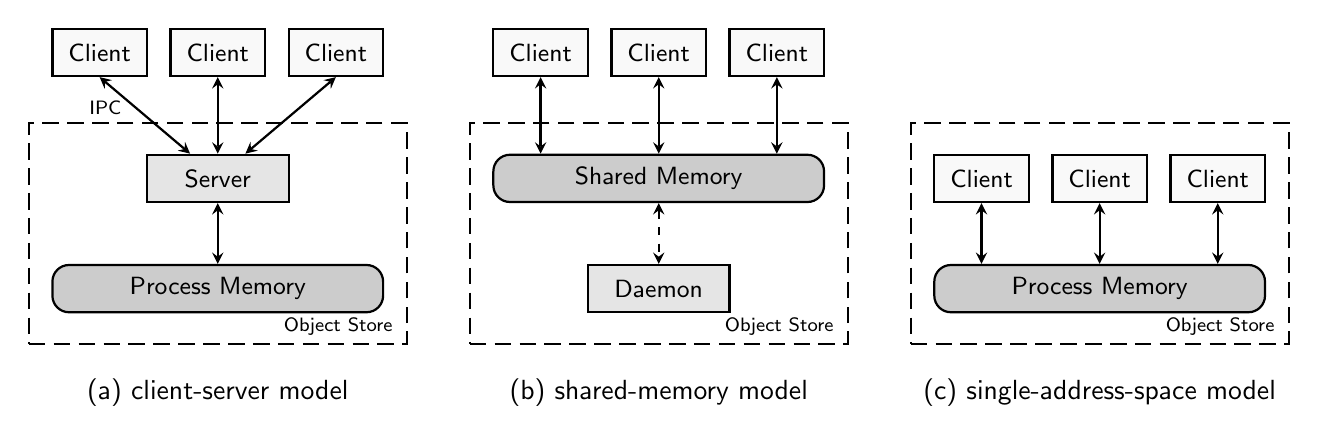
\begin{tikzpicture}[
				>=stealth,
				client/.style={rectangle, draw=black, thick, fill=gray!5, minimum width=1.2cm, minimum height=0.6cm, font=\sffamily\small},
				comp/.style={rectangle, draw=black, thick, fill=gray!20, minimum width=1.8cm, minimum height=0.6cm, font=\sffamily\small},
				memory/.style={rectangle, rounded corners=6pt, draw=black, thick, fill=gray!40, minimum width=4.2cm, minimum height=0.6cm, font=\sffamily\small},
				storebox/.style={draw=black, thick, dash pattern=on 6pt off 3pt, minimum width=4.8cm, minimum height=2.8cm},
				arr/.style={<->, thick},
				dasharr/.style={<->, dashed, thick}
			]

			\node[storebox] (a_store) at (0, -0.1) {};
			\node[storebox] (b_store) at (5.6, -0.1) {};
			\node[storebox] (c_store) at (11.2, -0.1) {};

			% Client-server
			\node[comp] (a_server) at (0, 0.6) {Server};
			\node[memory] (a_mem) at (0, -0.8) {Process Memory};
			\node[client] (a_c2) at (0, 2.2) {Client};
			\node[client] (a_c1) at (-1.5, 2.2) {Client};
			\node[client] (a_c3) at (1.5, 2.2) {Client};
			\draw[arr] (a_c1.south) -- ([xshift=-10pt]a_server.north);
			\draw[arr] (a_c2.south) -- (a_server.north);
			\draw[arr] (a_c3.south) -- ([xshift=10pt]a_server.north);
			\draw[arr] (a_server.south) -- (a_mem.north);
			\node[anchor=south east, font=\sffamily\scriptsize] at
			([xshift=-2pt,yshift=0pt]a_store.south east) {Object Store};
			\node[anchor=east, font=\sffamily\scriptsize] at (-1.1, 1.5) {IPC};
			\node[below=0.3cm of a_store, font=\sffamily] (cap_a) {(a) client-server model};

			% Shared memory
			\node[memory] (b_mem) at (5.6, 0.6) {Shared Memory};
			\node[comp] (b_daemon) at (5.6, -0.8) {Daemon};
			\node[client] (b_c2) at (5.6, 2.2) {Client};
			\node[client] (b_c1) at (4.1, 2.2) {Client};
			\node[client] (b_c3) at (7.1, 2.2) {Client};
			\draw[arr] (b_c1.south) -- (b_c1.south |- b_mem.north);
			\draw[arr] (b_c2.south) -- (b_mem.north);
			\draw[arr] (b_c3.south) -- (b_c3.south |- b_mem.north);
			\draw[dasharr] (b_mem.south) -- (b_daemon.north);
			\node[anchor=south east, font=\sffamily\scriptsize] at
			([xshift=-2pt,yshift=0pt]b_store.south east) {Object Store};
			\node[font=\sffamily] at (b_store.south |- cap_a) {(b) shared-memory model};

			% Single-address-space
			\node[client] (c_c2) at (11.2, 0.6) {Client};
			\node[client] (c_c1) at (9.7, 0.6) {Client};
			\node[client] (c_c3) at (12.7, 0.6) {Client};
			\node[memory] (c_mem) at (11.2, -0.8) {Process Memory};
			\draw[arr] (c_c1.south) -- (c_c1.south |- c_mem.north);
			\draw[arr] (c_c2.south) -- (c_mem.north);
			\draw[arr] (c_c3.south) -- (c_c3.south |- c_mem.north);
			\node[anchor=south east, font=\sffamily\scriptsize] at
			([xshift=-2pt,yshift=0pt]c_store.south east) {Object Store};
			\node[font=\sffamily] at (c_store.south |- cap_a) {(c) single-address-space
				model};

		\end{tikzpicture}
	\end{center}
    \caption{\label{fig:obj-store-arch} In-memory object store architectures.
    Figure inspired by Lightning~\cite{lightning22}.}
\end{figure*}

In-memory object stores allow independent programs to share live data without
the overhead of a disk write. While multi-threaded applications enable data
sharing by default (i.e., by memory reads and writes), \emph{multi-processed}
applications, where each component is executed in its own isolated process,
require specialized systems to communicate. Oftentimes, such architectures are
chosen to enable greater system security~\cite{reis19siteisolation} and fault
tolerance~\cite{wang19lineage}. For example, the Google Chrome browser renders
web sites in isolated processes to reduce the attack surface of malicious
JavaScript code~\cite{reis19siteisolation}. This use-case is incompatible with
single-address-space systems; in general, it is typical to trade performance for
security.

However, multi-process architectures may also be chosen for modularity (programs
can be developed and compiled independently) and convenience (programs can be
tested and run independently). In these settings, we wish to maintain the
benefits of \emph{logical} isolation, but depending on our security model and
performance requirements, it may be desirable to allow for greater data sharing
between programs. This motivates a design continuum, visualized in Figure
\ref{fig:obj-store-arch}, where object storage systems share increasing levels
of state.

\textbf{Client-server model.} In the client-server model, clients and the
database server are executed in isolated processes; they communicate over a
network or Unix socket. While this offers the strongest security
guarantees---namely that no process can corrupt the memory of any other
process---as described in Section \ref{sec:intro}, IPC overhead is significant
when executing all processes on the same machine.

\textbf{Shared-memory model.} Pioneered by Lightning~\cite{lightning22}, the
shared-memory model removes the designated server process and has clients
perform transactions directly upon a shared memory buffer. Using write-ahead
logging (WAL) and Intel Memory Protection Keys (MPK)~\cite{park19libmpk}, it is
still possible to maintain isolation: MPK protects internal database state from
faulty or malicious clients, and WAL ensures that transactions can be replayed
in the case of a client crash. However, in order to simplify formal
verification, Lightning uses a global spinlock to serialize transactions, and
since MPKs can be overwritten in user space, additional methods are required to
protect against actively malicious requirements. Thus, the shared-memory model
may be considered an intermediate between fully-isolated clients and
non-isolated clients.

\textbf{Single-address-space model.} In the single-address-space model, every
program executes within the same address address space (in Linux language, each
program is a \emph{thread} within the same \emph{process}). This simplifies
pointer-sharing and alleviates TLB pressure---a known bottleneck in
multi-processed systems~\cite{basu13bigmem, navarro02superpages}---at the cost of
process isolation. SAS-DB is the first single-address-space object store. Note
that although isolation is weaker than the shared-memory model (e.g., file
descriptors and signals are shared), Intel MPK can still be utilized to isolate
clients from the database and from each other. Even within the
single-address-space model, there are performance-isolation tradeoffs.

In this work, we operate within the single-address-space model due to its
potential for maximal performance.

\subsection{Concurrent Hash Tables}
\label{sec:hash-tables}
Since object stores typically expose a key-value interface and range queries
across objects are not semantically meaningful, hash tables are a natural fit
for scalable, low-latency queries. We borrow from a long line of work on
optimizing hash tables for high-concurrency. While several open-source
implementations are available
online,\footnote{\href{https://github.com/facebook/folly/blob/main/folly/concurrency/ConcurrentHashMap.h}{folly::ConcurrentHashMap},
	\href{https://github.com/divfor/atomic_hash}{atomic\_hash}} they are difficult
to adapt to specific use-cases and often introduce large software dependencies
(e.g., Facebook's Folly). As a result, our description focuses on techniques
rather than specific implementations.

\subsubsection{Lock Striping}
Rather than using a single, global lock to synchronize access to the entire hash
table, \emph{lock striping} partitions the table by key into an array of smaller
segments. Each segment is protected by a readers-writer
lock~\cite{herlihy20art}. In order to resize the table, one can acquire every
lock, or, alternatively, acquire an exclusive lock over the entire table. The
latter trades common-case latency for tail latency by introducing a shared
lock to every operation. Lock striping scales well so long as the hot segment
count exceeds the number of contending threads---in particular if the workload
is ready-heavy---but the per-operation atomic on the readers-writer lock remains
a fixed cost.

\subsubsection{Lock-free Chaining}
A concurrent data structure is \emph{lock-free} if some thread is guaranteed to
make progress in a bounded number of its own steps, so that no thread can stall
the system as a whole by being descheduled or crashing~\cite{herlihy91waitfree}.
While it is not true in general that lock-free algorithms outperform
locking-based ones, they often offer superior tail latency and concurrency
scaling. This makes them an obvious candidate for our use-cases.

In the absence of collisions, lock-free hash tables are very simple. One can
implement insertion with the following compare-and-swap loop:
\begin{verbatim}
while (!CAS(&table[hash(key)], ptr, expected)) {
    yield();
}
\end{verbatim}

A \texttt{get} simply performs an atomic read of the pointer
\texttt{\&table[hash(key)]}. Unfortunately, collisions are unavoidable, and
resolving them in a lock-free table is substantially more involved. We discuss
two influential designs. Michael's lock-free hash table~\cite{michael02highperf}
resolves collssion by chaining each bucket to a Harris-Michael lock-free linked
list~\cite{harris01lockfree}, with all of the insertion, lookup, and deletion
operations expressible as CASes on node pointers. Shalev and Shavit's
split-ordered list~\cite{shalev06splitorder} goes further and avoids rehashing
entries on resize: keys are stored in a single linked list whose order is
invariant under bucket-array growth, so resize updates pointers into the
list rather than moving entries. Our implementation uses the first design for
simplicity; note that since all of our values are pointers, copy overhead is not
quite as important.

\subsubsection{Safe Memory Reclamation}
Lock-free chaining introduces a subtle race condition during concurrent reads
and writes. Suppose that thread $t_{1}$ reads a value pointer $v$ just before
thread $t_{2}$ replaces it with $v'$. If $t_{2}$ were to immediately free the
memory pointed to by $v$, then $t_{1}$ would dereference a dangling pointer. A
partial solution is to use reference counting, so that $v$ will not be freed
until every reader decrements the ref-count. However, it is still possible that
$t_{2}$ overwrites $v$, decrements its ref-count to zero, and frees $v$ before
$t_{1}$ has a chance to increment the ref-count.

This problem also applies to the pointers internal to the data structure. A
thread that has just read a node pointer may dereference that pointer
arbitrarily later, so nodes cannot simply be freed once they are unliked. Safe
memory reclamation (SMR) schemes give threads a principled way to defer
reclamation of this memory until no concurrent reader can possibly hold a stale
reference~\cite{michael04hazard, hart07performance}.

\textbf{Epoch-based reclamation (EBR).} EBR~\cite{fraser04thesis} divides time
into coarse epochs. A thread announces the current epoch when it enters a
critical section and clears the announcement on exit; retired pointers
accumulate in per-thread free lists and are freed only once every active thread
has advanced past the epoch in which the pointer was retired. The fast path is
essentially free---a single relaxed store of the epoch number on entry---which
makes EBR attractive in benchmarks dominated by short, regular critical
sections. However, EBR makes strong assumptions regarding the liveness of
threads within a critical section: if an active thread stalls, reclamation is
deferred for \emph{all} threads, and memory growth is unbounded.

\textbf{Hazard pointers (HP).} HP~\cite{michael04hazard} tracks individual
pointer references rather than whole epochs. This allows the system to bound
memory consumption (i.e., $O(1)$ references per stalled thread) at the cost of a
slower fast-path. Each thread publishes, in a small set of per-thread slots, the
pointers it is currently dereferencing; a reclaimer scans these slots before
freeing and defers reclamation of any pointer still hazardous to some thread.
This requires a release-store and a re-read per protected dereference, leading
to potentially poor performance when many pointers must be protected in
sequence.

The choice between EBR and HP is typically informed by thread count and workload
regularity. The single-address-space setting changes both: client threads are
not introduced once at startup but at any time \emph{by the clients themselves}.
Since the database engine is not decoupled by client behavior, we must be
careful to account for adversarial client behavior, e.g., sudden
over-subscription due to thread spawns. This is pathological for EBR and
motivates our adoption of HP.

%-------------------------------------------------------------------------------
\section{Implementation}
%-------------------------------------------------------------------------------

We now describe the SAS-DB architecture in detail, including our design
decisions during implementation. In Section \ref{sec:eval-micro}, we provide
micro-benchmarks of system components to justify these choices. In Section
\ref{sec:eval-end-to-end}, we provide a comparison of Lightning with our most
well-rounded implementation.

Our system is a C++-23 prototype consisting of approximately 4500 lines of code.
While our client library is written in C, all of our tests and benchmarks are
written in C++ and we do not guarantee compatibility. We also provide a minimal
Java API for compatibility with YCSB~\cite{cooper10ycsb}.

\begin{figure}[ht]
\centering
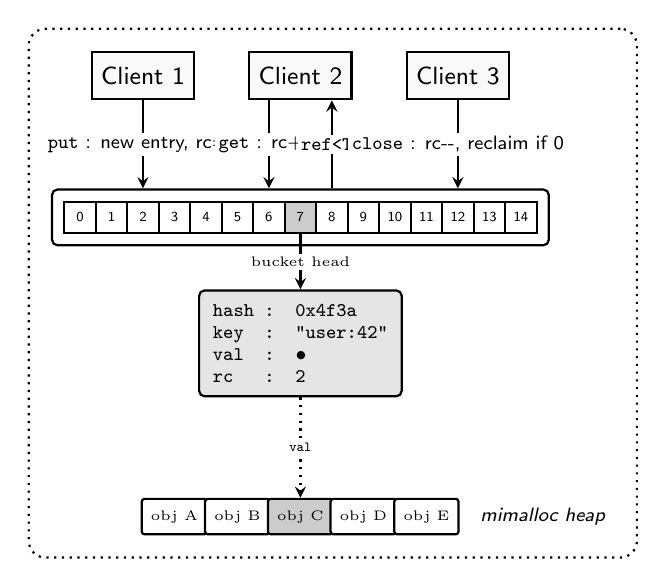
\begin{tikzpicture}[
    >=stealth,
    font=\sffamily\small,
    client/.style={rectangle, draw=black, thick, fill=gray!5, minimum width=1.2cm, minimum height=0.6cm, align=center},
    bucket/.style={rectangle, draw=black, thick, fill=white, minimum width=0.4cm, minimum height=0.4cm, font=\tiny\sffamily, inner sep=0pt},
    bucketHL/.style={bucket, fill=gray!40},
    entry/.style={rectangle, rounded corners=2pt, draw=black, thick, fill=gray!20, align=left, font=\scriptsize\ttfamily, inner sep=5pt},
    obj/.style={rectangle, rounded corners=1pt, draw=black, thick, fill=white, minimum width=0.6cm, minimum height=0.45cm, font=\tiny},
    objHL/.style={obj, fill=gray!40},
    arr/.style={->, thick},
    arrlbl/.style={font=\sffamily\scriptsize, fill=white, inner sep=1.2pt},
    process/.style={rectangle, rounded corners=6pt, draw=black, dotted, thick, inner sep=8pt}
]

\node[client] (c1) at (-2.0, 3.4) {Client 1};
\node[client] (c2) at ( 0.0, 3.4) {Client 2};
\node[client] (c3) at ( 2.0, 3.4) {Client 3};

\foreach \i in {0,...,14} {
    \pgfmathsetmacro{\xpos}{-2.8 + 0.4 * \i}
    \pgfmathtruncatemacro{\bidx}{\i}
    \node[bucket] (b\bidx) at (\xpos, 1.6) {\bidx};
}
\node[bucketHL] (bH) at (0, 1.6) {7};

\begin{pgfonlayer}{background}
    \node[draw=black, thick, rounded corners=2pt,
          inner sep=4pt, fit=(b0)(b14)] (hashTable) {};
\end{pgfonlayer}

\node[entry] (entry) at (0, 0.0) {%
    hash : \texttt{0x4f3a} \\
    key \ : "user:42" \\
    val \ : \(\bullet\)  \\
    rc \ \ : 2};

\draw[arr] (bH.south) -- (entry.north)
    node[arrlbl, pos=0.5, font=\tiny] {bucket head};

\node[obj] (oA) at (-1.6, -2.2) {obj A};
\node[obj] (oB) at (-0.8, -2.2) {obj B};
\node[objHL] (oC) at ( 0.0, -2.2) {obj C};
\node[obj] (oD) at ( 0.8, -2.2) {obj D};
\node[obj] (oE) at ( 1.6, -2.2) {obj E};

\node[font=\sffamily\scriptsize\itshape, anchor=west]
    (heapLabel) at ([xshift=4pt]oE.east)
    {mimalloc heap};

\draw[arr, dotted]
    (entry.south) -- (oC.north)
    node[arrlbl, pos=0.5, font=\tiny] {\texttt{val}};

\draw[arr] (c1.south) -- (c1.south |- hashTable.north)
    node[arrlbl, midway] {\texttt{put} : new entry, rc=1};

\draw[arr] ([xshift=-0.4cm]c2.south) --
    ([xshift=-0.4cm]c2.south |- hashTable.north)
    node[arrlbl, midway] {\texttt{get} : rc++};
\draw[arr] ([xshift=0.4cm]c2.south |- hashTable.north) --
    ([xshift=0.4cm]c2.south)
    node[arrlbl, midway] {\texttt{ref<T>}};

\draw[arr] (c3.south) -- (c3.south |- hashTable.north)
    node[arrlbl, midway] {\texttt{close} : rc-{}-, reclaim if 0};

\begin{pgfonlayer}{background}
    \node[process,
        fit=(c1)(c3)(hashTable)(entry)(oA)(heapLabel)]
        (proc) {};
\end{pgfonlayer}
\end{tikzpicture}
\caption{\label{fig:backend-arch} Backend of SAS-DB. Clients read and write
directly to a concurrent hash table. Values initially have ref-count 1, which is
incremented and decremented on \texttt{get} and \texttt{close}, respectively.
Clients use a shared mimalloc heap.}
\end{figure}

\subsection{Client Loading}
At startup, Lightning executes the \emph{host} binary which is responsible for
loading client programs. Currently, our system takes as input a list of files
corresponding to client binaries (which must be \texttt{-fPIC} shared
libraries); these are then loaded using \texttt{dlopen} and a distinguished
\texttt{entry} function is called from a new thread. The host sleeps until every
client terminates; unlike Lightning, there is no daemon.

In order to support dynamic process invocation, an alternative design is to read
client binary names from a Unix socket. This has no performance implications
except that the host must monitor for new clients to launch. We have not
implemented this yet simply because it is not relevant to benchmarking.

\subsection{Client API}
Since clients are loaded as shared libraries, they have access to host code via
symbol resolution. We provide the following API to clients (as a single-header
include \texttt{client.h}) which dynamically executes host code at runtime:
\begin{itemize}
    \item \texttt{get(key) $\to$ handle*}: Get from a key (which may be any
    C-string). Rather than returning values directly, this function returns an
    opaque handle which must be \emph{dereferenced} using the following
    operator.
    \item \texttt{deref(handle*) $\to$ void*}: Dereference a handle to obtain a
    \emph{value pointer}. All data types stored within SAS-DB are 8-byte
    pointers. This allows clients to define their own value representations,
    e.g., arrays of fields or pointer-based trees.
    \item \texttt{close(handle*)}: Decrement the ref-count of a handle.
    Necessary to prevent memory leaks.
    \item \texttt{put(key, value*, dtor)}: Store a value pointer at the location
    referenced by \texttt{key} and register a \emph{destructor} to be called
    when the value's ref-count reaches zero. This function takes ownership of
    \texttt{value} via \texttt{dtor}.
\end{itemize}

\subsubsection{Reference Counting}
The decision to use reference counting for values was not made lightly. Since
every value needs a corresponding handle, a handle must be allocated on every
\texttt{put}. In addition, the atomic increment and decrement on every
\texttt{get} and \texttt{close} can lead to frequent cache coherence misses
under heavy contention. Unfortunately, every alternative either reduces API
flexibility or performance. For example, a visitation-based API would need to
hold locks (or stay within a EBR or HP critical section) while executing client
callbacks. This leads to a clunky programming model for database queries, which
often depend on the result of previous queries.

In order to mitigate these performance concerns, we use
mimalloc~\cite{leijen19mimalloc}, a general-purpose allocator optimized for
concurrent, ref-count-heavy workloads. In addition, we maintain a thread-local
pool of handle allocations that are used when possible; freed handles return
directly to the pool until it reaches capacity.

\subsubsection{C++ Library}
In addition to the more general C API, we provide a C++ convenience library that
uses the RAII pattern and templates for simpler programming. For example,
storing and retrieving an integer uses the following syntax, where \texttt{close}
is automatic:
\begin{verbatim}
void entry() {
    auto value = std::make_unique<int>(2640);
    sas::put("example", value);
    auto handle = sas::get("example");
    assert(*value == *handle);
}
\end{verbatim}

The client entry-point \texttt{entry} will always succeed without an assertion
failure or memory leak; the \texttt{handle} object can be dereferenced similarly
to a raw value; and the value destructor is passed within the type of
\texttt{std::unique\_ptr}.

\subsection{Backend}
The database itself is a concurrent hash table much like the strategies
discussed in Section \ref{sec:hash-tables}. We provide five modular backends
which are benchmarked extensively in Section \ref{sec:eval-micro}:

\textbf{Spinlock.} A naive implementation based on C++'s
\texttt{std::unordered\_map} with a spinlock for synchronization. This is our
baseline (and performs similarly to Lightning).

\textbf{Sharded.} A highly-optimized implementation of lock striping based on
\texttt{boost::concurrent\_flat\_map}. Unlike chaining-based solutions, the
sharded backend uses open addressing and SIMD-accelerated probing. Uses a
stop-the-world approach to resizing with exclusive locks.

\textbf{Lock-free (EBR).} A lock-free implementation using chaining and EBR for
reclamation. Supports cooperative resizing.

\textbf{Lock-free (HP).} A lock-free implementation using chaining and HP for
reclamation. Supports cooperative resizing.

\textbf{Hybrid.} A further optimized form of the sharded backend that performs
writes (i.e., value pointer CASes) while holding a \emph{read} lock rather than
a write lock. This is only possible because SAS-DB stores exclusively pointer
types (which, in turn, is a consequence of the shared-address-space model).
However, HP must still be used to protect value pointers before incrementing the
ref-count.

Despite the complexity of the lock-free solutions, we find that the hybrid
backend performs best under the most varied situations. As a result, it is the
default in our codebase.

\section{Evaluation}
\label{sec:eval}

We evaluate SAS-DB along two axes. In Section~\ref{sec:eval-micro} we use
microbenchmarks to (i) compare the five hash table backends introduced in
Section~\ref{sec:hash-tables}, (ii) isolate the architectural contribution of
the single-address-space model, and (iii) measure the overhead added by the
SAS-DB client API on top of the raw backend. In
Section~\ref{sec:eval-end-to-end} we compare SAS-DB end-to-end against
Lightning on the YCSB benchmark.

All experiments run on a single CloudLab node with a two-way SMT Intel Xeon (24
physical cores at 2.795~GHz, 32~KiB L1, 512~KiB L2, 16~MiB shared L3 across each
6-core slice). Frequency scaling is disabled. Both SAS-DB and Lightning are
compiled with \texttt{-O3} under C++23 and linked against
mimalloc~\cite{leijen19mimalloc}. Unless otherwise noted, microbenchmarks use $N
= 2^{22}$ keys, a 50\% read / 50\% write mix, Zipfian access with $\theta =
0.99$, and report steady-state aggregate throughput from Google Benchmark.
Latency statistics come from per-thread histograms merged at the end of each
run.

For YCSB, we use the Java workload generator from the upstream YCSB
distribution~\cite{cooper10ycsb}. SAS-DB hosts a single multi-threaded JVM as a
client, while Lightning runs the default multi-process recipe in which each
client process is its own JVM and the keyspace is partitioned across processes.
Although a partitioned keyspace is highly favorable to a concurrent system, we
were unable to run Lightning's benchmarking code on non-partitioned keys.

\subsection{Microbenchmarks}
\label{sec:eval-micro}

\subsubsection{Backend Comparison}
Figure~\ref{fig:backends-thr} reports read-write throughput for the five
backends as the client thread count is swept from $T = 1$ to 64. The spinlock
baseline collapses immediately: serializing every operation through a single
critical section, throughput drops below half of its single-threaded value at
two threads and below 1\% of its single-threaded value by sixteen threads. This
motivates our implementation of complex, multi-threaded data structures to
eliminate this scaling bottleneck.

The two lock-free chained backends (EBR and HP) perform similarly across the
sweep until $T = 64$, when EBR suddenly collapses. Although this may appear to
be experimental noise, we have reproduced this effect with multiple reruns; it
is well-known that EBR underperforms when threads are frequently
preempted~\cite{nikolaev21snapshot}, such as when threads are oversubscribed.
While HP performs very well overall, our implementation does not currently have
support for deletion, which requires much heavier atomic operations while
traversing each chain. The sharded backend is faster than EBR/HP at low thread
counts---SIMD-accelerated probing in \texttt{boost::concurrent\_flat\_map}
dominates---but loses that advantage once contention increases.

Figure~\ref{fig:backends-keys} reports read-write throughput as the number of
keys is swept from $N = 2^{11}$ to $2^{24}$. Although the lock-free backends
perform significantly better at low key counts (possibly because they resize
more aggressively than the sharded backend), at $N = 2^{24}$ every backend
except for spinlock performs similarly at about 1.5~Mops/s.

The hybrid backend, which performs every pointer CAS while holding only a
read lock, meets or exceeds every other backend at high thread counts and
high key counts. We adopt it as SAS-DB's default.

\begin{figure}[t]
    \centering
    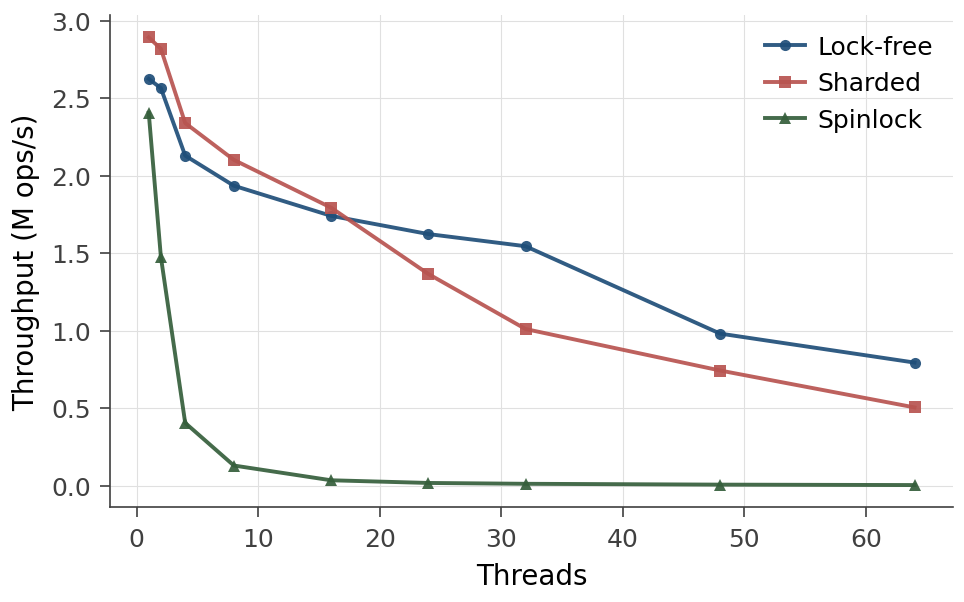
\includegraphics[width=\columnwidth]{../results/backends/num_threads/mixed_throughput.png}
    \caption{\label{fig:backends-thr} Mixed-workload throughput of the five
    SAS-DB backends as a function of client thread count ($N = 2^{22}$, 50/50
    read/write, Zipfian $\theta = 0.99$).}
\end{figure}
\begin{figure}[t]
    \centering
    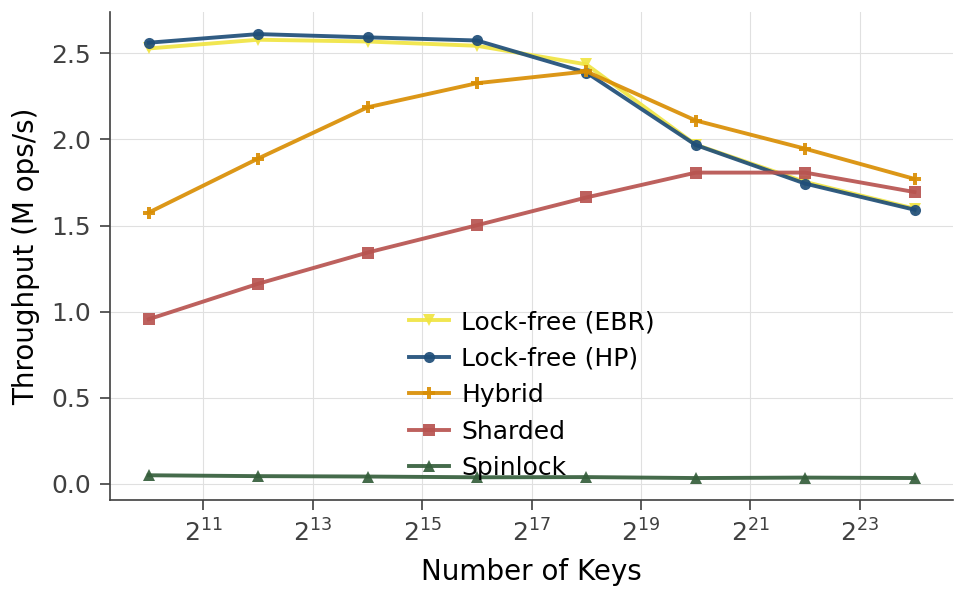
\includegraphics[width=\columnwidth]{../results/backends/num_keys/mixed_throughput.png}
    \caption{\label{fig:backends-keys} Mixed-workload throughput of the five
    SAS-DB backends as a function of the key count ($T = 16$, 50/50 read/write,
    Zipfian $\theta = 0.99$).}
\end{figure}

\subsubsection{Architecture Comparison}
\label{sec:eval-arch}
To isolate the architectural contribution of the single-address-space model, we
run two builds that differ only in where the store memory lives. The SAS build
uses a standard shared heap; the SHM build maps a POSIX shared memory region
into a leader process and a varying number of worker processes. In order to
minimize reimplementation, we make use of mimalloc's \emph{arena} feature, which
allows users to provide pre-allocated heap regions (in this case, the shared
memory buffer). While this suffices for benchmarking purposes, there is no
support for cross-process \texttt{free}s, so we use a read-only workload. In
addition, cross-process locking (i.e., for the hybrid backend) does not work, so
both builds use the HP backend and the same workload generator.

\begin{figure}[t]
    \centering
    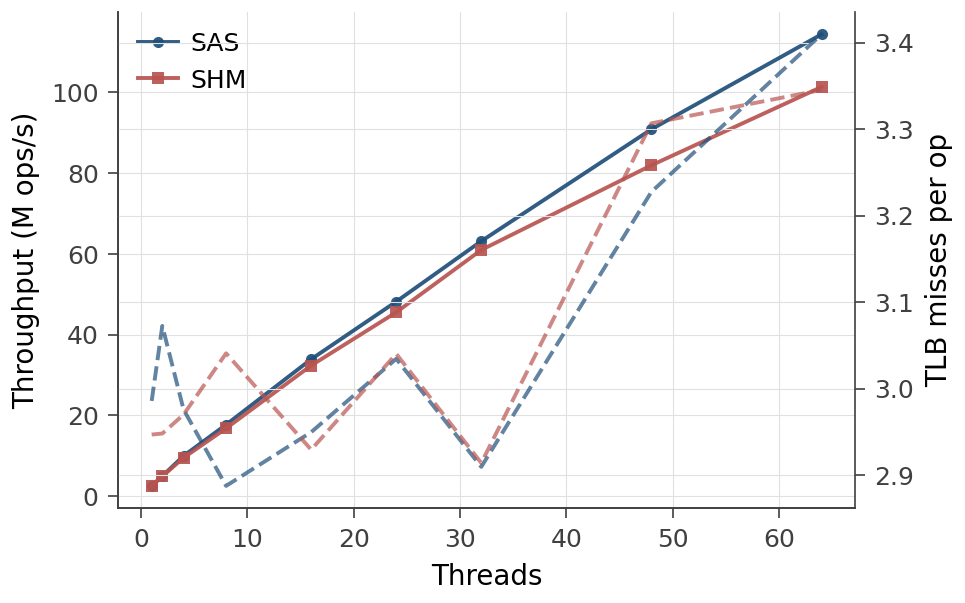
\includegraphics[width=\columnwidth]{../results/arch/num_threads/mixed_throughput.png}
    \caption{\label{fig:arch-thr} SAS-DB versus an otherwise-identical
    shared-memory build, as a function of client thread count. The right-hand
    axis reports per-op L2 TLB misses, sampled with \texttt{perf}.}
\end{figure}

Up to about 24 threads---the physical core count---the two configurations
track each other within roughly 2\%. Beyond that point, the workload saturates
the available cores and processes begin to evict one another's TLB entries: the
SHM build's per-operation page-walk count climbs sharpy (from 0.23 and 24
threads to 0.76 at 64 threads) as 64 distinct page tables walk the same data.
The SAS build, sharing a single page table, sustains the same access pattern at
0.51 page walks per operation. The throughput gap follows the same trend: at 64
threads, SAS reaches 85.2~Mops/s vs. 75.7~Mops/s for SHM, a 12.4\% improvement.
That is close to 10 million additional ops/s attributable to collapsing the
multi-process boundary alone.

\subsubsection{Client API Overhead}
The microbenchmarks above operate directly against the chosen backend. In order
to sanity-check that dynamic loading and symbol resolution does not affect
performance, we compare the native hybrid backend against the end-to-end SAS-DB
stack on the same workload (i.e., the benchmark program is loaded as a shared
library as opposed to linking \texttt{hybrid\_store.cpp}). The end-to-end stack
sustains throughput within a small factor of the native backend across the sweep
and reports a read p99 of 1.20~$\mu$s and a write p99 of 1.37~$\mu$s. This is
significantly more robust than comparable systems such as Lightning.

\begin{figure}[t]
    \centering
    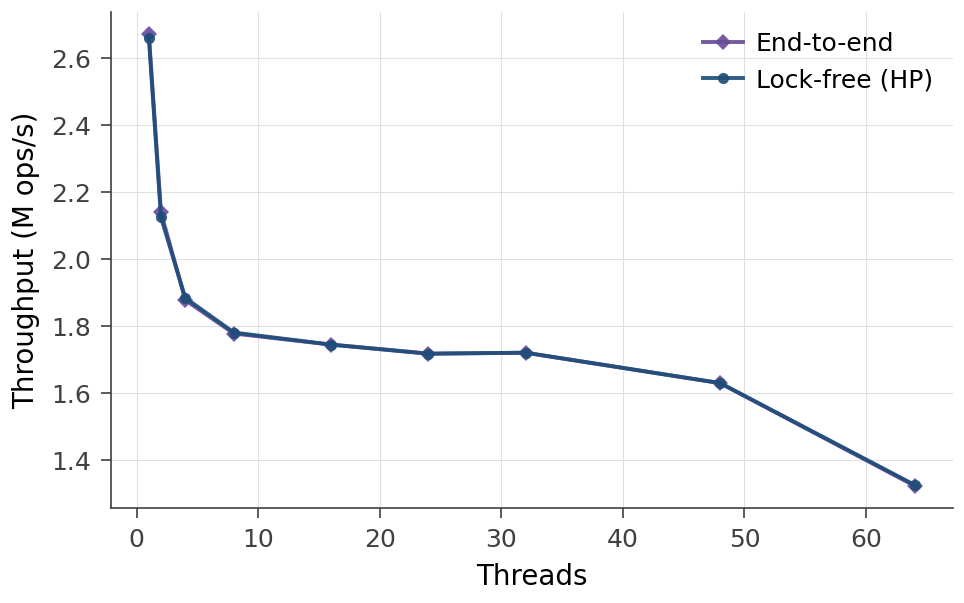
\includegraphics[width=\columnwidth]{../results/client_overhead/num_threads/mixed_throughput.png}
    \caption{\label{fig:client-overhead} Throughput of the native hybrid backend
    versus the end-to-end SAS-DB stack. Both run the same workload.}
\end{figure}

\begin{figure}[t]
    \centering
    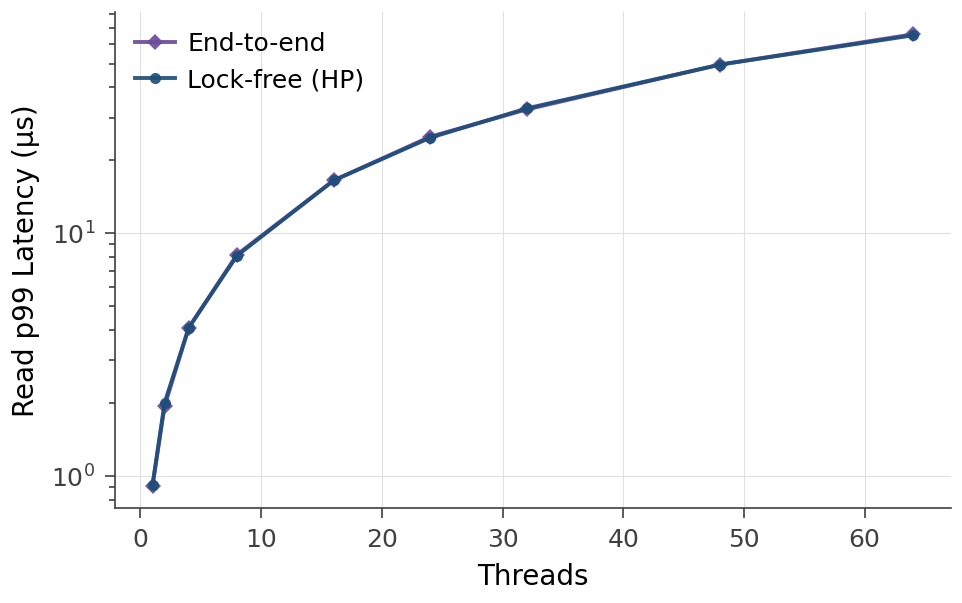
\includegraphics[width=\columnwidth]{../results/client_overhead/num_threads/mixed_rd_p99.png}
    \caption{\label{fig:client-overhead-rd} P99 read latency of the native
    hybrid backend versus the end-to-end SAS-DB stack. Both run the same
    workload.}
\end{figure}

\begin{figure}[t]
    \centering
    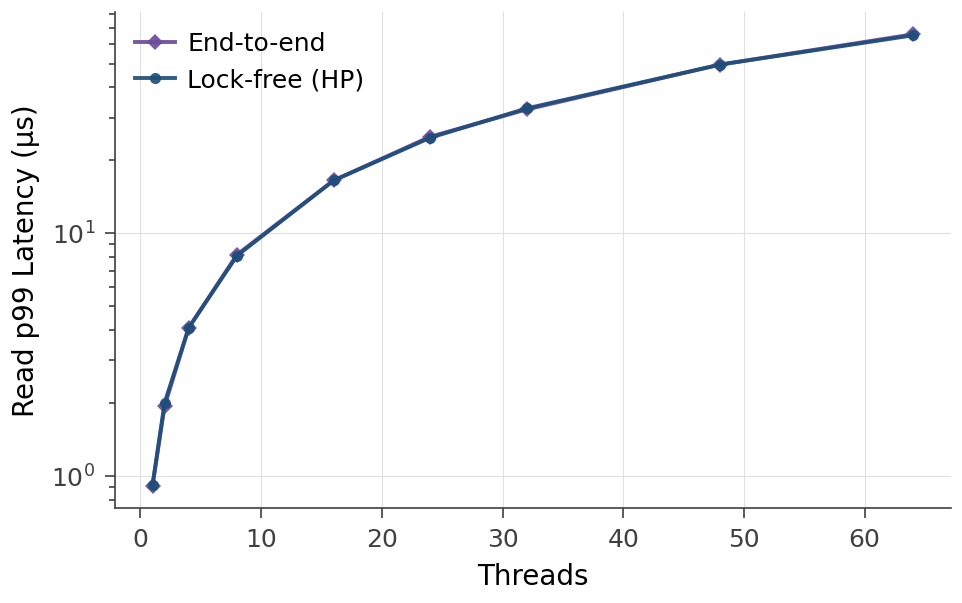
\includegraphics[width=\columnwidth]{../results/client_overhead/num_threads/mixed_rd_p99.png}
    \caption{\label{fig:client-overhead-wr} P99 write latency of the native
    hybrid backend versus the end-to-end SAS-DB stack. Both run the same
    workload.}
\end{figure}

\subsection{End-to-End Benchmarks}
\label{sec:eval-end-to-end}

We compare SAS-DB to Lightning on the Yahoo! Cloud Serving
Benchmark~\cite{cooper10ycsb}. We run YCSB workloads A, B, C, D, and F at 1, 2,
4, and 8 client threads (although SAS-DB can support higher thread counts, the
runtime of Lightning is prohibitively slow). Workload E (range scans) is omitted
because neither system supports range queries. As described in the setup,
Lightning runs in its recommended multi-process configuration with a partitioned
keyspace, and SAS-DB runs as a single multi-threaded JVM client linked into the
host.

\begin{table}[t]
    \centering
    \small
    \begin{tabular}{lrrrrr}
                                 & A     & B    & C    & D    & F     \\ \hline
        SAS-DB (8 threads)       & 1.42  & 1.43 & 1.52 & 1.29 & 1.04  \\
        Lightning (8 threads)    & 0.12  & 0.22 & 0.27 & 0.24 & 0.10  \\ \hline
        Speedup ($\times$)       & 12.1  & 6.5  & 5.7  & 5.5  & 10.4  \\
    \end{tabular}
    \caption{\label{tab:ycsb-8} YCSB run-phase throughput in Mops/s at 8
        client threads. Workload E omitted (no range scans).}
\end{table}

\begin{figure}[t]
    \centering
    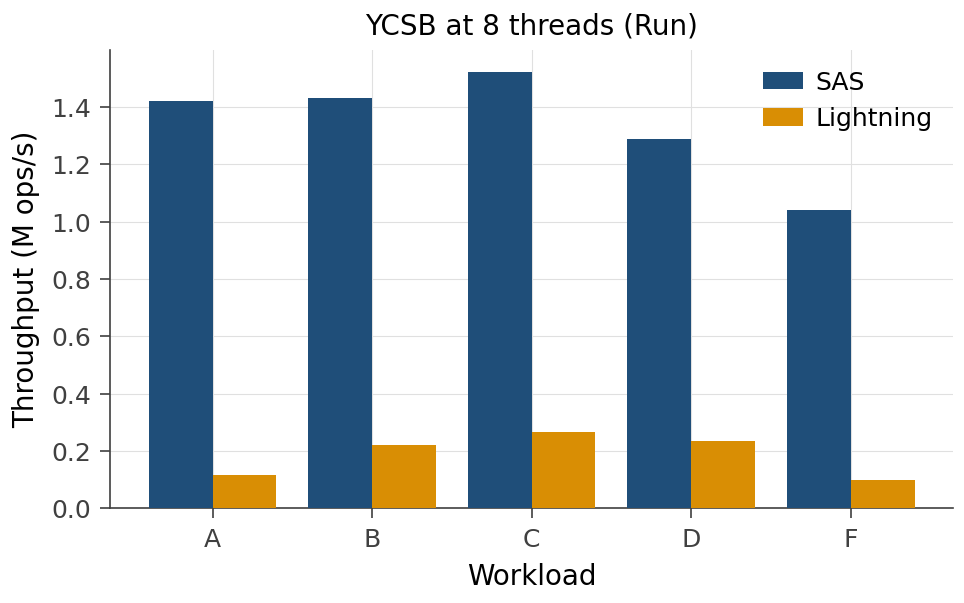
\includegraphics[width=\columnwidth]{../results/ycsb/threads_8_run.png}
    \caption{\label{fig:ycsb-8-run} YCSB run-phase throughput at 8 client
        threads, SAS-DB versus Lightning.}
\end{figure}

SAS-DB outperforms Lightning on every workload at every thread count we tested.
The smallest 8-thread speedup, 5.7$\times$, occurs on the read-only workload C,
which is the closest case to Lightning's best published configuration. The
largest, 12.1$\times$, occurs on the 50/50 mixed workload A, where Lightning's
global spinlock serializes both reads and writes. Two characteristics of the
data are worth highlighting. First, SAS-DB's run-phase throughput grows roughly
linearly with thread count: across the workload set, 8-thread throughput
averages $3.8\times$ the single-threaded throughput, which is expected for a
concurrent hash table with partitioned queries. Second, Lightning's run-phase
throughput is essentially flat: its 8-thread numbers are within $\pm 15\%$ of
its 1-thread numbers across all five workloads, consistent with the spinlock
contention discussed in Section~\ref{sec:intro}. The gap therefore widens
monotonically with thread count, and SAS-DB's advantage is not the result of a
particular workload but the underlying scaling behavior.

\section{Conclusion}

We presented SAS-DB, an in-memory key-value store that loads its clients as
shared libraries into a single flat address space. Doing so eliminates both the
IPC boundary that traditional client-server stores rely on for communication and
the multi-process boundary that shared-memory stores rely on for isolation. On
YCSB, SAS-DB outperforms Lightning by between $5.7$x and $12.1$x at eight client
threads; on a microbenchmark that isolates the single-address-space
contribution alone, the same hash table sustains $12.4\%$ more throughput than
an otherwise-identical shared-memory build at 64 threads. We also found that the
right concurrency primitives in this settings are not the conventional ones:
Epoch-based reclamation, commonly preferred for short-lived critical sections
like hash table reads, is unsuited to a workload in which client threads spawn
and stall outside of the engine's control. A simple hybrid scheme that performs
pointer CAS while holding a read lock matches or beats every fully lock-free
backend we implemented. We hope that the design choices and pitfalls documented
here are useful for future single-address-space systems, and that the
substantial performance overhead we measured motivates revisiting the
long-standing assumption that intra-server object stores must isolate clients in
separate processes.

%-------------------------------------------------------------------------------
\bibliographystyle{plain}
\bibliography{usenix2019_v3.1}

%%%%%%%%%%%%%%%%%%%%%%%%%%%%%%%%%%%%%%%%%%%%%%%%%%%%%%%%%%%%%%%%%%%%%%%%%%%%%%%%
\end{document}
%%%%%%%%%%%%%%%%%%%%%%%%%%%%%%%%%%%%%%%%%%%%%%%%%%%%%%%%%%%%%%%%%%%%%%%%%%%%%%%%
